In this section we report on the application of the proposed method for surveillance strategy synthesis on gridworld-based examples. The purpose of the experimental evaluation is to highlight the following key points:
\begin{itemize}
    \item The effect of different abstractions on the evolution of the belief sets of the agent.
    \item Sequences of abstractions resulting from automated abstraction refinement.
    \item The qualitative differences in the agent's behaviour resulting from surveillance strategies synthesized for different types of specifications.
\end{itemize}


We apply the \texttt{slugs} reactive synthesis tool~\cite{EhlersR16} to the abstract surveillance games in order to synthesize the surveillance strategies. The experiments were performed on an Intel i5-5300U 2.30 GHz CPU with 8 GB of RAM. 

\subsection{Effect of Abstractions on Belief}
The aim of this experiment is to illustrate the effect of different abstractions (generated using different abstraction partitions) on the evolution of belief sets. Naturally, the finer the abstraction, the slower the growth of the size of the belief set over time, and hence the easier it is to satisfy the specification. However, the increased precision of the abstraction comes at the cost of increased synthesis time. 

Figure~\ref{fig:case1} shows a gridworld divided into 7 abstraction partitions. The surveillance objective requires the agent to infinitely often know precisely the location of the target (either see it, or have a belief consisting of one cell). Additionally, it has to perform the task of patrolling (visiting infinitely often) the green 'goal' cell. Formally, the specification is $\LTLglobally\LTLfinally p_1 \wedge \LTLglobally\LTLfinally \mathit{goal}$. The agent can move up to 3 grid cells away at each step. The sensor mode, that is, the observation function, used here is 'line-of-sight' with a range of 5 cells. The agent cannot see through obstacles (shown in red) and cannot see farther than 5 cells away.  We assume in this example that we have perfect sensing i.e., when the target is sensed, the agent knows its true location. There are no static sensors. 


\begin{figure}
\subfloat[Gridworld with a user-provided abstraction partition with 7 sets, marked by the thick black lines. \label{fig:case1}]{
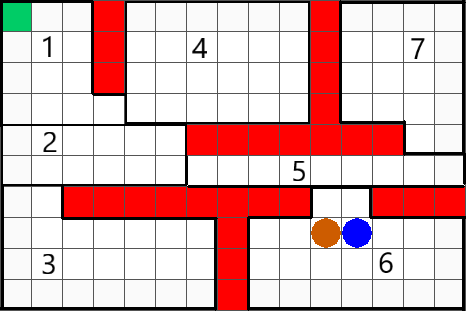
\includegraphics[width=0.45\linewidth]{Surveillance/figs/Liveness_part.png}
}
\hfill
\subfloat[Gridworld showing visibility of the agent. All locations shown in black are invisible to the agent. \label{fig:case1vis}]{
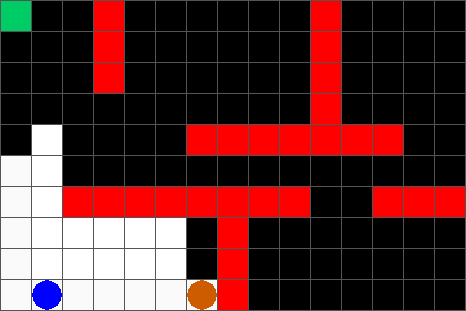
\includegraphics[width=0.45\linewidth]{Surveillance/figs/Liveness_t1.png}
}

\caption{10x15 gridworld with a liveness surveillance specification. The agent is depicted in blue, and the target in orange. The red locations are obstacles.}
\label{fig:casestudies1}

\end{figure}



\begin{figure}
\begin{minipage}{5.0cm}
	\centering
		\subfloat[$t_1$ \label{fig:case1t2}]{
		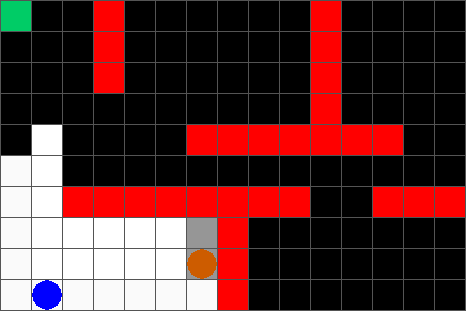
\includegraphics[width=0.47\linewidth]{Surveillance/figs/Liveness_t2.png}\hspace{.5cm}
	}
	\subfloat[$t_3$ \label{fig:case1t3}]{
		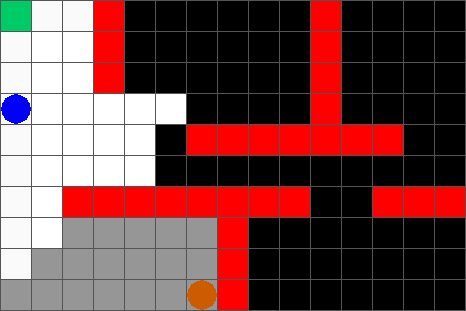
\includegraphics[width=0.47\linewidth]{Surveillance/figs/Liveness_t3.png}\hspace{.5cm}
	}
	\subfloat[$t_4$ \label{fig:case1t4}]{
	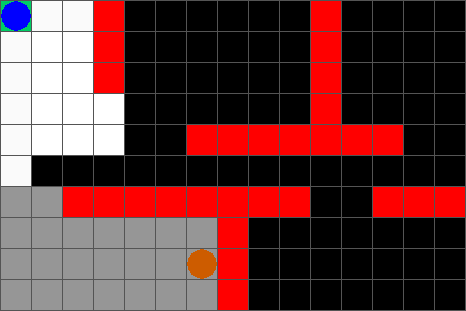
\includegraphics[width=0.47\linewidth]{Surveillance/figs/Liveness_t4.png}\hspace{.5cm}
}
\end{minipage}
\begin{minipage}{5.0cm}
	\centering
	\subfloat[$t_5$  \label{fig:case1t5}]{
		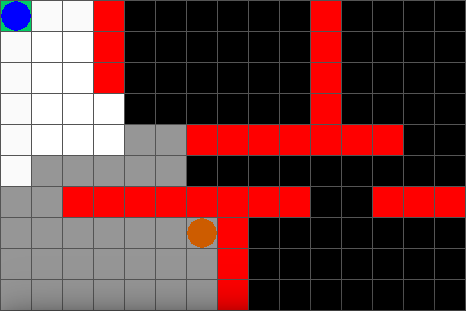
\includegraphics[width=0.47\linewidth]{Surveillance/figs/Liveness_t5.png}\hspace{.5cm}
	}
	\subfloat[$t_6$ \label{fig:case1t6}]{
		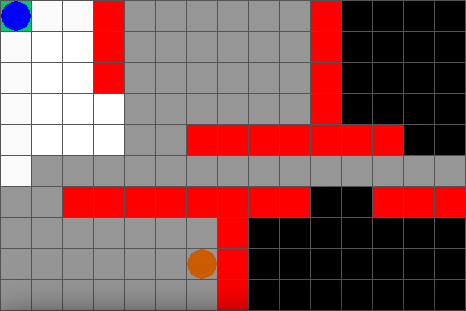
\includegraphics[width=0.47\linewidth]{Surveillance/figs/Liveness_t6.png}\hspace{.5cm}
	}
	\subfloat[$t_7$ \label{fig:case1t7}]{
		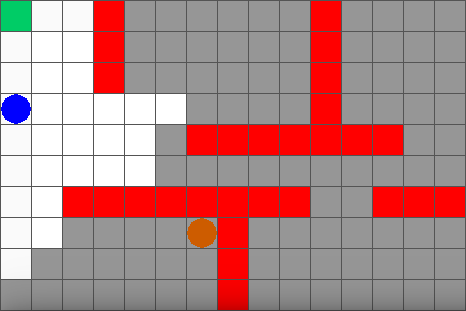
\includegraphics[width=0.47\linewidth]{Surveillance/figs/Liveness_t7.png}\hspace{.5cm}
	}
	
\end{minipage}

	
	\caption{Evolution of the agent's belief about the target's location as it moves towards the goal and loses sight of the target. Grey cells represent the locations the agent believes the target could be in. We show the belief at different timesteps $t_1,\ldots,t_7$ (note that $t_2$ is excluded for space concerns)
		}
	\label{fig:case1exp}
	
\end{figure}

Figure \ref{fig:case1exp} shows how the belief of the agent (shown in grey) can grow quickly when it cannot see the target. This growth occurs due to the coarseness of the abstraction, which overapproximates the target's true location. In 7 steps, the agent believes the target can be anywhere in the grid that is not in its vision. It has to then find the target in order to satisfy the surveillance requirement. Figure \ref{fig:search} illustrates the searching behaviour of the agent when it is trying to lower the belief below the threshold in order to satisfy the liveness specification. This  behaviour contrasts with the behaviour under safety surveillance considered later. A video of the simulation can be found at \url{http://goo.gl/YkFuxr}.

\begin{figure}

	\begin{minipage}{5.0cm}
		\centering
		\subfloat[$t_5$ \label{fig:search1}]{
			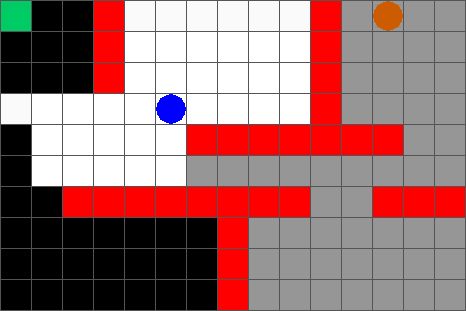
\includegraphics[width=0.47\linewidth]{Surveillance/figs/search_t2.png}\hspace{.5cm}
		}
		\subfloat[$t_7$ \label{fig:search2}]{
			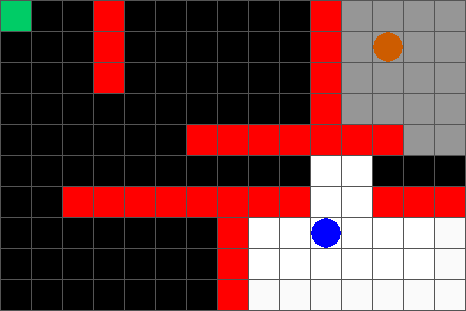
\includegraphics[width=0.47\linewidth]{Surveillance/figs/search_t3.png}\hspace{.5cm}
		}
		\subfloat[$t_9$ \label{fig:search3}]{
			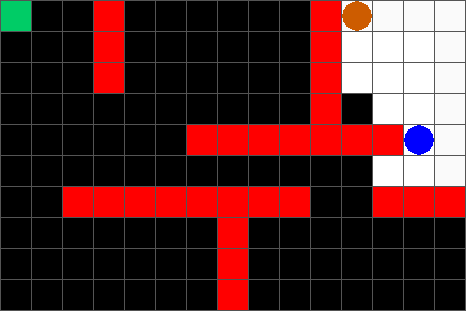
\includegraphics[width=0.47\linewidth]{Surveillance/figs/search_t4.png}\hspace{.5cm}
		}
	\end{minipage}
	\caption{The agent has to search for the target in order to lower its belief below the surveillance liveness specification.
	}
	\label{fig:search}
	
\end{figure}

In this example, an abstraction partition of size 7 was enough to guarantee the satisfaction of the surveillance specification.  For the purpose of comparison, we also solve the game with  an abstraction partition of size 12  to illustrate the change in belief growth. Figure \ref{fig:case1fineexp} shows the belief states growing much more slowly as the abstract belief states are smaller, and thus they more closely  approximate the true belief.
\begin{figure}

	\begin{minipage}{5.0cm}
		\centering
		\subfloat[$t_1$ \label{fig:casefine1t2}]{
			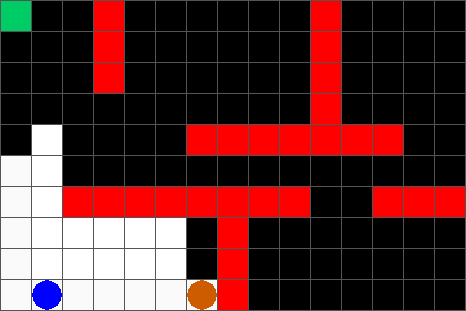
\includegraphics[width=0.47\linewidth]{Surveillance/figs/Liveness_t1.png}\hspace{.5cm}
		}
		\subfloat[$t_3$ \label{fig:case1finet3}]{
			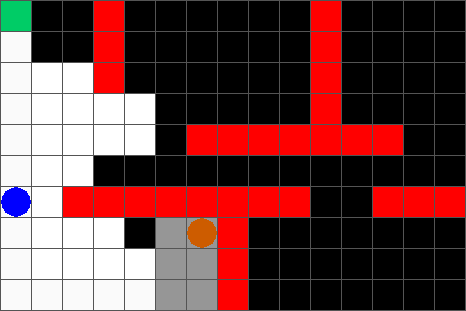
\includegraphics[width=0.47\linewidth]{Surveillance/figs/Liveness_fine_t11.png}\hspace{.5cm}
		}
		\subfloat[$t_4$ \label{fig:case1finet4}]{
			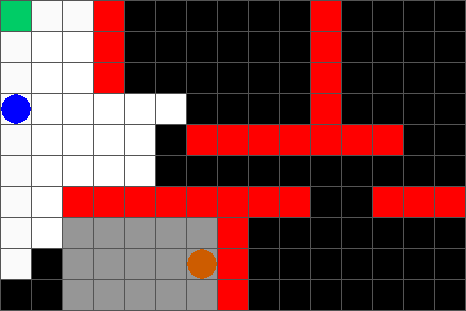
\includegraphics[width=0.47\linewidth]{Surveillance/figs/Liveness_fine_t2.png}\hspace{.5cm}
		}
	\end{minipage}
	\begin{minipage}{5.0cm}
		\centering
		\subfloat[$t_5$  \label{fig:case1finet5}]{
			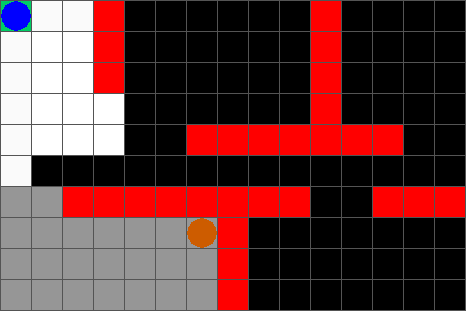
\includegraphics[width=0.47\linewidth]{Surveillance/figs/Liveness_fine_t3.png}\hspace{.5cm}
		}
		\subfloat[$t_6$ \label{fig:case1finet6}]{
			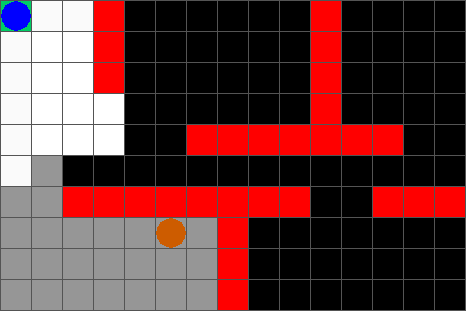
\includegraphics[width=0.47\linewidth]{Surveillance/figs/Liveness_fine_t4.png}\hspace{.5cm}
		}
		\subfloat[$t_7$ \label{fig:case1finet7}]{
			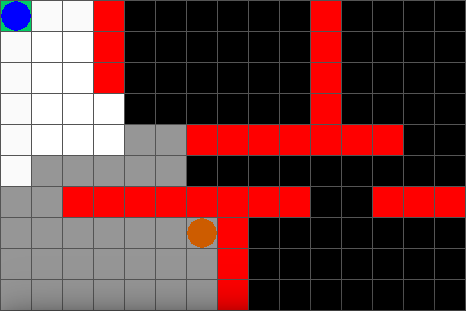
\includegraphics[width=0.47\linewidth]{Surveillance/figs/Liveness_t5.png}\hspace{.5cm}
		}
		
	\end{minipage}
	
	
	\caption{Evolution of the agent's belief about the target's location in a game  with an abstraction partition of size 12.
	}
	\label{fig:case1fineexp}
	
\end{figure}


The additional abstraction partitions result in a much larger game as the state space grows exponentially in the size of the abstraction partition. We compared the sizes of two abstract games for the 15x10 gridworld shown in Figure \ref{fig:casestudies1}, and the time it takes to synthesize a surveillance strategy in each of them. For an abstraction partition of size 7 the abstract game has 41700 states, and the synthesis time is 237s. In comparison, for an abstraction partition of size 13 the size of the abstract game is 636900 and the synthesis time is 810s. In contrast, the concrete belief-set game will have in the order of $2^{150}$ states, which is a state-space size that state-of-the-art synthesis tools cannot handle. 

%Table \ref{tab:exp1} compares the sizes of the corresponding abstract games, and the time it takes to synthesize a surveillance controller in each case.


%\begin{table}[h!]
%	\centering
%	\begin{tabular}{c|c|c}
%	Size of abstraction partition & Size of abstract game & Synthesis time \\ \hline \hline
%		7 & 41700 & 237s \\ 
%		12 & 636900 & 810s \\ 
%	\end{tabular}\caption{Comparison of synthesis times for coarse and fine abstractions on a 15x10 gridworld shown in Figure \ref{fig:casestudies}} \label{tab:exp1}
%\end{table}




\subsection{Automated Abstraction Refinement}
We now present an experiment to demonstrate the working of abstraction refinement procedure. 


\begin{figure}
\subfloat[User-provided initial abstraction. \label{fig:case1_autopart_before}]{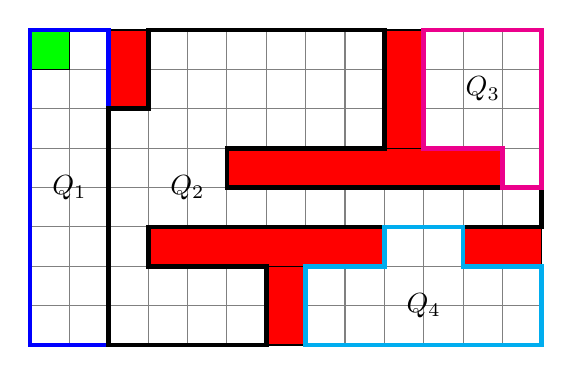
\begin{tikzpicture}[scale=1]
\draw[step=0.5cm,color=gray] (-3.5,-2) grid (3,2);


\filldraw[fill=green,draw=black] (-3.5,2) rectangle (-3,1.5);
% \filldraw[fill=red,draw=black] (-2.5,2) rectangle (-2,1.5);
\filldraw[fill=red,draw=black] (-2.5,2) rectangle (-2,1.0);
\filldraw[fill=red,draw=black] (1,2) rectangle (1.5,0.0);
\filldraw[fill=red,draw=black] (-1,0.5) rectangle (2.5,0.0);
\filldraw[fill=red,draw=black] (2,-0.5) rectangle (3,-1.0);
\filldraw[fill=red,draw=black] (-2,-0.5) rectangle (1,-1.0);
\filldraw[fill=red,draw=black] (-0.5,-1.0) rectangle (0,-2.0);

\filldraw[fill=none,draw=blue,line width=0.6mm] (-3.5,2.0) rectangle (-2.5,-2.0);
\draw[black, line width = 0.6mm] plot coordinates{(-2.0,2) (-2.0,1) (-2.5,1) (-2.5,-2) (-0.5,-2) (-0.5,-1) (-2.0,-1) (-2.0,-0.5) (3.0,-0.5) (3.0,-0.0) (-1.0,-0.0) (-1.0,0.5) (1.0,0.5) (1.0,2)}--cycle;
\draw[cyan, line width = 0.6mm] plot coordinates{(0,-1.0) (0,-2.0) (3,-2.0) (3,-1.0) (2,-1.0) (2,-0.5) (1,-0.5) (1,-1.0)}--cycle;
\draw[magenta, line width = 0.6mm] plot coordinates{(1.5,2.0) (1.5,0.5) (2.5,0.5) (2.5,0.0) (3.0,0.0) (3.0,2.0)}--cycle;
% \filldraw[fill=blue!40!white,draw=black] (+0.75,+0.75) circle (0.2cm);
% \filldraw[fill=orange!40!white,draw=black] (0.25,-0.75) circle (0.2cm);
\node at (-3.0,+0.0) {\normalsize{\textbf{$Q_1$}}};
\node at (-1.5,-0.0) {\normalsize{\textbf{$Q_2$}}};
\node at (2.25,1.25) {\normalsize{\textbf{$Q_3$}}};
\node at (1.5,-1.5) {\normalsize{\textbf{$Q_4$}}};
% \node at (-1.5,-0.0) {\large{\textbf{2}}};
% \node at (-0.30,+0.75) {\tiny{2}};
% \node at (0.20,+0.75) {\tiny{3}};
% \node at (0.73,+0.75) {\tiny{4}};
% \node at (-1.33,+0.25) {\tiny{5}};
% \node at (-0.85,+0.25) {\tiny{6}};
% \node at (-0.35,+0.25) {\tiny{7}};
% \node at (0.25,+0.25) {\tiny{8}};
% \node at (0.75,+0.25) {\tiny{9}};
% \node at (-1.28,-0.27) {\tiny{10}};
% \node at (-0.78,-0.27) {\tiny{11}};
% \node at (-0.28,-0.27) {\tiny{12}};
% \node at (0.28,-0.27) {\tiny{13}};
% \node at (0.75,-0.25) {\tiny{14}};
% \node at (-1.3,-0.75) {\tiny{15}};
% \node at (-0.8,-0.75) {\tiny{16}};
% \node at (-0.3,-0.75) {\tiny{17}};
% \node at (0.25,-0.75) {\tiny{18}};
% \node at (0.75,-0.75) {\tiny{19}};
% \node at (-1.27,-1.25) {\tiny{20}};
% \node at (-0.8,-1.25) {\tiny{21}};
% \node at (-0.3,-1.25) {\tiny{22}};
% \node at (0.25,-1.25) {\tiny{23}};
% \node at (0.75,-1.25) {\tiny{24}};
\end{tikzpicture}}
%\hfill
\subfloat[Refined abstraction.\label{fig:refined-abstraction}]{
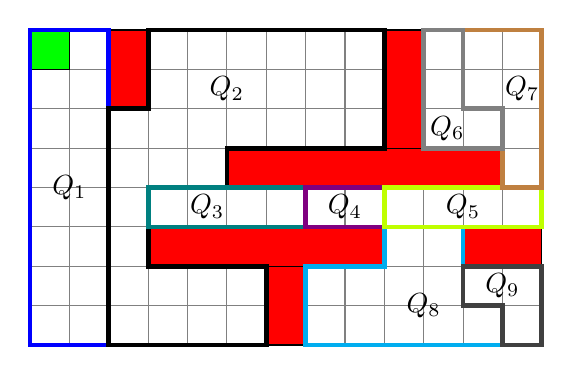
\begin{tikzpicture}[scale=1]
\draw[step=0.5cm,color=gray] (-3.5,-2) grid (3,2);


\filldraw[fill=green,draw=black] (-3.5,2) rectangle (-3,1.5);
% \filldraw[fill=red,draw=black] (-2.5,2) rectangle (-2,1.5);
\filldraw[fill=red,draw=black] (-2.5,2) rectangle (-2,1.0);
\filldraw[fill=red,draw=black] (1,2) rectangle (1.5,0.0);
\filldraw[fill=red,draw=black] (-1,0.5) rectangle (2.5,0.0);
\filldraw[fill=red,draw=black] (2,-0.5) rectangle (3,-1.0);
\filldraw[fill=red,draw=black] (-2,-0.5) rectangle (1,-1.0);
\filldraw[fill=red,draw=black] (-0.5,-1.0) rectangle (0,-2.0);

\filldraw[fill=none,draw=blue,line width=0.6mm] (-3.5,2.0) rectangle (-2.5,-2.0);
\draw[black, line width = 0.6mm] plot coordinates{(-2.0,2) (-2.0,1) (-2.5,1) (-2.5,-2) (-0.5,-2) (-0.5,-1) (-2.0,-1) (-2.0,-0.0) (-1.0,-0.0) (-1.0,0.5) (1.0,0.5) (1.0,2)}--cycle;
\draw[cyan, line width = 0.6mm] plot coordinates{(0,-1.0) (0,-2.0) (3,-2.0) (3,-1.0) (2,-1.0) (2,-0.5) (1,-0.5) (1,-1.0)}--cycle;


\filldraw[fill=none,draw=teal, line width=0.6mm] (-2.0,0.0) rectangle (-0.0,-0.5);
\filldraw[fill=none,draw=violet, line width=0.6mm] (-0.0,0.0) rectangle (1.0,-0.5);
\filldraw[fill=none,draw=lime, line width=0.6mm] (1.0,0.0) rectangle (3.0,-0.5);
\draw[brown, line width = 0.6mm] plot coordinates{(2.0,2.0) (2.0,1.0) (2.5,1.0) (2.5,0.0) (3.0,0.0) (3.0,2.0)}--cycle;
\draw[gray, line width = 0.6mm] plot coordinates{(1.5,2.0) (1.5,0.5) (2.5,0.5) (2.5,1.0) (2.0,1.0) (2.0,2.0)}--cycle;
\draw[darkgray, line width = 0.6mm] plot coordinates{(2.0,-1.0) (2.0,-1.5) (2.5,-1.5) (2.5,-2.0) (3,-2.0) (3,-1)}--cycle;


% \filldraw[fill=blue!40!white,draw=black] (+0.75,+0.75) circle (0.2cm);
% \filldraw[fill=orange!40!white,draw=black] (0.25,-0.75) circle (0.2cm);
\node at (-3.0,+0.0) {\textbf{$Q_1$}};
\node at (-1.25,-0.25) {\normalsize{\textbf{$Q_3$}}};
\node at (-1.0,1.25) {\normalsize{\textbf{$Q_2$}}};
\node at (1.5,-1.5) {\normalsize{\textbf{$Q_8$}}};
\node at (0.5,-0.25) {\normalsize{\textbf{$Q_4$}}};
\node at (2.0,-0.25) {\normalsize{\textbf{$Q_5$}}};
\node at (1.8,0.75) {\normalsize{\textbf{$Q_6$}}};
\node at (2.75,1.25) {\normalsize{\textbf{$Q_7$}}};
\node at (2.5,-1.25) {\normalsize{\textbf{$Q_9$}}};
% \node at (-1.5,-0.0) {\large{\textbf{2}}};
% \node at (-0.30,+0.75) {\tiny{2}};
% \node at (0.20,+0.75) {\tiny{3}};
% \node at (0.73,+0.75) {\tiny{4}};
% \node at (-1.33,+0.25) {\tiny{5}};
% \node at (-0.85,+0.25) {\tiny{6}};
% \node at (-0.35,+0.25) {\tiny{7}};
% \node at (0.25,+0.25) {\tiny{8}};
% \node at (0.75,+0.25) {\tiny{9}};
% \node at (-1.28,-0.27) {\tiny{10}};
% \node at (-0.78,-0.27) {\tiny{11}};
% \node at (-0.28,-0.27) {\tiny{12}};
% \node at (0.28,-0.27) {\tiny{13}};
% \node at (0.75,-0.25) {\tiny{14}};
% \node at (-1.3,-0.75) {\tiny{15}};
% \node at (-0.8,-0.75) {\tiny{16}};
% \node at (-0.3,-0.75) {\tiny{17}};
% \node at (0.25,-0.75) {\tiny{18}};
% \node at (0.75,-0.75) {\tiny{19}};
% \node at (-1.27,-1.25) {\tiny{20}};
% \node at (-0.8,-1.25) {\tiny{21}};
% \node at (-0.3,-1.25) {\tiny{22}};
% \node at (0.25,-1.25) {\tiny{23}};
% \node at (0.75,-1.25) {\tiny{24}};
\end{tikzpicture}
}
\caption{Experiment showcasing automated abstraction refinement in a 13$\times$8 gridworld. The user-provided abstraction of 4 abstract states shown in ~\ref{fig:case1_autopart_before} is refined further into 9 abstract states shown in~\ref{fig:refined-abstraction}.}
\label{fig:case1_autopart}
\end{figure}



Starting with an abstract game generated by a partition with four elements shown in Figure~\ref{fig:case1_autopart_before}, the refinement algorithm terminates after 5 iterations (with total running time of 821 s). The resulting partition $\mathcal{Q} = \{Q_1,...,Q_9 \}$ has $9$ elements shown as the numbered regions in Figure~\ref{fig:refined-abstraction}.

This experiment shows that, in general, we do not guarantee that the abstraction generated by the refinement approach is necessarily the smallest possible. A handcrafted partitioning in the same environment shown in the previous section was able to produce a winning strategy with 7 abstract belief states instead of 9. Although the abstraction refinement algorithm is always guaranteed to terminate, in general, the user-provided initial abstraction has a significant effect on the number of abstract belief states of the resulting abstraction. It is thus important to combine initial user-provided abstractions, that are crafted as well as possible, with the automated refinement that eliminates any remaining imprecision that was not accounted for by the user.

 



%\Suda{Not sure if we should keep this next part}
\subsection{Discussion}
 The difference in the behaviour in the case studies highlights the different use cases of the surveillance objectives. Depending on the domain, the user can specify a combination of safety and liveness specification to tune the behaviour of the agent. In a critical surveillance situation (typical in defense or security situations), the safety specification will guarantee to the user that the belief will never grow too large. However, in less critical situations (such as luggage carrying robots in airports), the robot has more flexibility in allowing the belief to grow as long as it can guarantee its reduction in the future. 